\documentclass[12pt,a4paper]{article}
\usepackage[utf8]{inputenc}
\usepackage[spanish]{babel}
\usepackage{geometry}
\geometry{left=2.5cm,right=2.5cm,top=3cm,bottom=3cm}
\usepackage{graphicx}
\usepackage{hyperref}
\usepackage{fancyhdr}
\usepackage{titlesec}
\usepackage{xcolor}
\usepackage{listings}
\usepackage{enumitem}
\usepackage{amssymb}
\usepackage{float}

% Encabezados y pies de página
\pagestyle{fancy}
\fancyhf{}
\fancyhead[L]{Pontificia Universidad Católica del Ecuador}
\fancyhead[R]{Manual del Sistema}
\fancyfoot[C]{\thepage}

% Títulos destacados
\titleformat{\section}
  {\normalfont\Large\bfseries\color{teal}}{\thesection}{1em}{}
\titleformat{\subsection}
  {\normalfont\large\bfseries\color{black}}{\thesubsection}{1em}{}

% Configuración para bloques de código
\lstset{
    backgroundcolor=\color{gray!10},
    frame=single,
    basicstyle=\ttfamily\footnotesize,
    breaklines=true,
    keywordstyle=\color{blue}\bfseries,
    commentstyle=\color{gray}\it,
    stringstyle=\color{orange},
    showstringspaces=false,
    numbers=left,
    numberstyle=\tiny,
    xleftmargin=1em,
    xrightmargin=1em,
    tabsize=4
}

\begin{document}

% Portada
\begin{titlepage}
\begin{flushright}   
 \vspace*{-2cm}
 
\includegraphics[height=2.5cm]{Imagenes/logo puce.png} 
\end{flushright}
 \centering
 \vspace*{1cm}
 {\Huge\bfseries Manual del Sistema\\[1.5ex] \textit{Mis Gastos}}\\[2cm]
 {\Large Pontificia Universidad Católica del Ecuador}\\[1cm]
 {\large Carrera: Tec Desarrollo De Software}\\[0.5cm]
 {\large Asignatura: Programación II}\\[0.5cm]
 {\large Profesor: Kevin Viteri}\\[1cm]
 {\large Elaborado por:}\\[0.3cm]
 {\bfseries Ariel Rosero y Ahinoa Andino}\\[2cm]
 {\large Quito, \today}
 \vfill
\end{titlepage}

\tableofcontents
\newpage

\section{Introducción}
Este manual es una guía paso a paso para crear el sistema \textbf{Mis Gastos} usando Django, permitiendo registrar, visualizar y administrar tus gastos personales. Cada sección explica con detalle los comandos, archivos y estructura del proyecto, asegurando que cualquier persona pueda replicarlo y obtener exactamente el mismo resultado.

\section{Requisitos previos}
Antes de empezar, verifica que tienes instalado:
\begin{itemize}
    \item \textbf{Python 3.9 o superior}
    \item \textbf{pip} (gestor de paquetes de Python)
    \item \textbf{Un editor de código} (VS Code, PyCharm, Sublime Text, etc.)
    \item \textbf{Git} (opcional)
    \item \textbf{Navegador web}
\end{itemize}
\textbf{Consejo:} Trabaja siempre en un \textbf{entorno virtual} para evitar problemas de dependencias.

\section{¿Qué es cada carpeta y archivo?}
\begin{tabular}{|l|l|}
\hline
Archivo/Carpeta & Descripción \\
\hline
manage.py & Comando principal para gestionar Django \\
misgastos/ & Configuración global del proyecto Django \\
gastos/ & Nuestra app principal para gastos \\
gastos/templates/gastos/ & Archivos HTML (plantillas) de la app \\
gastos/static/gastos/ & Archivos CSS y JS de la app \\
db.sqlite3 & Base de datos local de Django \\
.venv/ & Entorno virtual de Python \\
\hline
\end{tabular}

\section{Creación manual de carpetas esenciales}
Django NO crea automáticamente las carpetas de plantillas ni estáticos en la app. Debes crearlas así:
\begin{lstlisting}[language=bash]
mkdir -p gastos/templates/gastos
mkdir -p gastos/static/gastos
\end{lstlisting}
\textbf{Nota:} En Windows, usa el explorador o:
\begin{lstlisting}[language=bash]
mkdir gastos\templates\gastos
mkdir gastos\static\gastos
\end{lstlisting}

\section{Creación del proyecto y entorno de trabajo}

\subsection{1. Crear carpeta y entorno virtual}
\begin{enumerate}
    \item Abre la terminal y ejecuta:
    \begin{lstlisting}[language=bash]
    mkdir mis-gastos
    cd mis-gastos
    python -m venv .venv
    \end{lstlisting}
    \item Activa el entorno virtual:
    \begin{itemize}
        \item En Windows:
        \begin{lstlisting}[language=bash]
        .venv\Scripts\activate
        \end{lstlisting}
        \item En Mac/Linux:
        \begin{lstlisting}[language=bash]
        source .venv/bin/activate
        \end{lstlisting}
    \end{itemize}
\end{enumerate}

\subsection{2. Instalar Django}
\begin{lstlisting}[language=bash]
pip install django
\end{lstlisting}

\subsection{3. Crear el proyecto Django}
\begin{lstlisting}[language=bash]
django-admin startproject misgastos .
\end{lstlisting}

\subsection{4. Crear la aplicación}
\begin{lstlisting}[language=bash]
python manage.py startapp gastos
\end{lstlisting}

\subsection{5. Estructura de carpetas esperada}
\begin{lstlisting}
mis-gastos/
├─ misgastos/
│   ├─ __init__.py
│   ├─ asgi.py
│   ├─ settings.py
│   ├─ urls.py
│   └─ wsgi.py
├─ gastos/
│   ├─ __init__.py
│   ├─ admin.py
│   ├─ apps.py
│   ├─ migrations/
│   ├─ models.py
│   ├─ tests.py
│   ├─ views.py
│   └─ (otros archivos)
├─ manage.py
└─ .venv/
\end{lstlisting}

\section{Configuración inicial}

\subsection{1. Registrar la app en \texttt{settings.py}}
Abre \texttt{misgastos/settings.py} y en \texttt{INSTALLED\_APPS} añade:
\begin{lstlisting}[language=Python]
INSTALLED_APPS = [
    # apps de django
    'gastos',  # nuestra app
]
\end{lstlisting}

\subsection{2. Configurar archivos estáticos}
En el mismo archivo, define:
\begin{lstlisting}[language=Python]
STATIC_URL = '/static/'
import os
STATICFILES_DIRS = [
    os.path.join(BASE_DIR, 'gastos/static'),
]
\end{lstlisting}

\section{Modelos y base de datos}

\subsection{1. Definir el modelo de gastos}
En \texttt{gastos/models.py}:
\begin{lstlisting}[language=Python]
from django.db import models

class Gasto(models.Model):
    descripcion = models.CharField(max_length=120)
    monto = models.DecimalField(max_digits=10, decimal_places=2)
    fecha = models.DateField(auto_now_add=True)

    def __str__(self):
        return f"{self.descripcion}: ${self.monto}"
\end{lstlisting}

\subsection{2. Migrar la base de datos}
\begin{lstlisting}[language=bash]
python manage.py makemigrations
python manage.py migrate
\end{lstlisting}

\section{Vistas y rutas}

\subsection{1. Crear las vistas}
En \texttt{gastos/views.py}:
\begin{lstlisting}[language=Python]
from django.shortcuts import render, redirect
from .models import Gasto
from django.db.models import Sum

def landing(request):
    gastos_count = Gasto.objects.count()
    total_gastado = Gasto.objects.aggregate(total=Sum('monto'))['total'] or 0
    return render(request, 'gastos/landing.html', {
        'gastos_count': gastos_count,
        'total_gastado': f"{total_gastado:.2f}"
    })

def formulario_gasto(request):
    if request.method == "POST":
        descripcion = request.POST.get("descripcion")
        monto = request.POST.get("monto")
        if descripcion and monto:
            Gasto.objects.create(descripcion=descripcion, monto=monto)
            return redirect('listado_gastos')
    return render(request, 'gastos/formulario.html')

def listado_gastos(request):
    gastos = Gasto.objects.all().order_by('-fecha')
    return render(request, 'gastos/listado.html', {"gastos": gastos})
\end{lstlisting}

\subsection{2. Definir las rutas de la app}
Crea \texttt{gastos/urls.py}:
\begin{lstlisting}[language=Python]
from django.urls import path
from . import views

urlpatterns = [
    path('', views.landing, name='landing'),
    path('agregar/', views.formulario_gasto, name='formulario_gasto'),
    path('historial/', views.listado_gastos, name='listado_gastos'),
]
\end{lstlisting}

\subsection{3. Rutas del proyecto}
En \texttt{misgastos/urls.py}:
\begin{lstlisting}[language=Python]
from django.contrib import admin
from django.urls import path, include

urlpatterns = [
    path('admin/', admin.site.urls),
    path('', include('gastos.urls')),
]
\end{lstlisting}

\section{Plantillas HTML}

Crea la carpeta \texttt{gastos/templates/gastos/}. Allí, agrega los siguientes archivos:

\subsection{1. landing.html}
\begin{lstlisting}[language=HTML]
<!DOCTYPE html>
<html lang="es">
<head>
    <meta charset="UTF-8">
    <title>Mis Gastos - Inicio</title>
    <link rel="stylesheet" href="/static/gastos/style.css">
</head>
<body>
    <div class="hero-content">
        <h1>Controla tus gastos<br>y alcanza tus metas</h1>
        <p>Lleva un seguimiento claro y ágil de todos tus movimientos.</p>
        <a href="" class="btn-principal">Empieza ahora</a>
        <p>Total gastado: ${{ total_gastado }}</p>
        <p>Gastos registrados: {{ gastos_count }}</p>
        <a href="">Ver historial</a>
    </div>
</body>
</html>
\end{lstlisting}

\subsection{2. formulario.html}
\begin{lstlisting}[language=HTML]
<!DOCTYPE html>
<html lang="es">
<head>
    <meta charset="UTF-8">
    <title>Agregar gasto</title>
    <link rel="stylesheet" href="/static/gastos/style.css">
    <script src="/static/gastos/scrips.js" defer></script>
</head>
<body>
    <form id="gastoForm" action="" method="post" class="form-gasto">
        
        <div class="campo-form">
            <label for="descripcion">Descripción</label>
            <input type="text" name="descripcion" id="descripcion" required>
        </div>
        <div class="campo-form">
            <label for="monto">Monto gastado</label>
            <input type="number" step="0.01" name="monto" id="monto" required>
        </div>
        <div id="form-message"></div>
        <button type="submit" class="btn-principal">Agregar Gasto</button>
    </form>
    <a href="">Ver historial</a>
</body>
</html>
\end{lstlisting}

\subsection{3. listado.html}
\begin{lstlisting}[language=HTML]
<!DOCTYPE html>
<html lang="es">
<head>
    <meta charset="UTF-8">
    <title>Historial de gastos</title>
    <link rel="stylesheet" href="/static/gastos/style.css">
</head>
<body>
    <h2>Historial de gastos</h2>
    <ul class="gastos-list">
        
            <li class="gasto-item">
                <span class="descripcion">{{ gasto.descripcion }}</span>
                <span class="monto">${{ gasto.monto }}</span>
                <span class="fecha">{{ gasto.fecha }}</span>
            </li>
        
            <li class="gasto-vacio">No hay gastos registrados aún.</li>
        
    </ul>
    <a href="">Agregar nuevo gasto</a>
</body>
</html>
\end{lstlisting}

\section{Archivos estáticos}

Crea la carpeta \texttt{gastos/static/gastos/} y agrega:

\subsection{1. style.css}
\begin{lstlisting}[language=CSS]
body {
    background: #f4f7fb;
    font-family: 'Inter', Arial, sans-serif;
    color: #253245;
    margin: 0;
    padding: 0;
}
.hero-content {
    text-align: center;
    margin-top: 60px;
}
.btn-principal {
    background: linear-gradient(90deg, #1abc9c 0%, #19857b 100%);
    color: #fff;
    border-radius: 28px;
    font-size: 1.25rem;
    font-weight: 700;
    border: none;
    padding: 10px 25px;
    margin-top: 20px;
    cursor: pointer;
}
.form-gasto {
    max-width: 400px;
    margin: 40px auto;
    background: #fff;
    border-radius: 10px;
    padding: 25px 30px;
    box-shadow: 0 5px 25px rgba(0,0,0,0.06);
}
.campo-form {
    margin-bottom: 18px;
}
.campo-form label {
    display: block;
    margin-bottom: 6px;
    font-weight: 600;
}
.campo-form input {
    width: 100%;
    padding: 8px;
    border-radius: 5px;
    border: 1px solid #ddd;
    font-size: 1rem;
}
.gastos-list {
    list-style: none;
    padding: 0;
    max-width: 450px;
    margin: 40px auto;
}
.gasto-item {
    background: #eaf0f6;
    border-radius: 8px;
    padding: 10px 15px;
    margin-bottom: 10px;
    display: flex;
    justify-content: space-between;
    align-items: center;
}
\end{lstlisting}

\subsection{2. scrips.js}
\begin{lstlisting}[language=JavaScript]
document.addEventListener('DOMContentLoaded', function () {
    // Validación y feedback en el formulario de gasto
    const form = document.getElementById('gastoForm');
    const msg = document.getElementById('form-message');
    if (form && msg) {
        form.addEventListener('submit', function (e) {
            const descripcion = form.descripcion.value.trim();
            const monto = parseFloat(form.monto.value);
            if (!descripcion || isNaN(monto) || monto <= 0) {
                e.preventDefault();
                msg.textContent = "Por favor escribe una descripción válida y un monto mayor a 0.";
                msg.style.color = "#d32f2f";
                return false;
            }
        });
    }
});
\end{lstlisting}

\section{Panel de administración (opcional)}

\begin{enumerate}
    \item Crear usuario administrador:
    \begin{lstlisting}[language=bash]
    python manage.py createsuperuser
    \end{lstlisting}
    \item Registrar el modelo en \texttt{gastos/admin.py}:
    \begin{lstlisting}[language=Python]
    from django.contrib import admin
    from .models import Gasto

    admin.site.register(Gasto)
    \end{lstlisting}
    \item Accede a \url{http://127.0.0.1:8000/admin} usando tu usuario admin.
\end{enumerate}

\section{Ejecución y pruebas}

\subsection{1. Ejecutar el servidor}
\begin{lstlisting}[language=bash]
python manage.py runserver
\end{lstlisting}
Abre tu navegador y accede a: \url{http://127.0.0.1:8000/}

\subsection{2. Estructura final de carpetas}
\begin{lstlisting}
mis-gastos/
├─ misgastos/
├─ gastos/
│  ├─ migrations/
│  ├─ static/gastos/
│  │  ├─ style.css
│  │  └─ scrips.js
│  ├─ templates/gastos/
│  │  ├─ landing.html
│  │  ├─ formulario.html
│  │  └─ listado.html
│  ├─ models.py, views.py, urls.py, admin.py, ...
├─ Imagenes/
│  ├─ Manual_MisGastos_Definitivo.tex
│  ├─ logo puce.png
│  ├─ Pagina Principal.png
│  ├─ Formulario.png
│  └─ Historial de gastos.png
├─ manage.py
├─ db.sqlite3
\end{lstlisting}

\section{¿Dónde colocar las imágenes de evidencia?}
Guarda tus capturas de pantalla dentro de la carpeta \texttt{Imagenes/}. Ejemplo:
\begin{lstlisting}
Imagenes/
├─ logo puce.png
├─ Pagina Principal.png
├─ Formulario.png
├─ Historial de gastos.png
\end{lstlisting}
Luego, llama las imágenes así en tu manual:
\begin{lstlisting}[language=TeX]
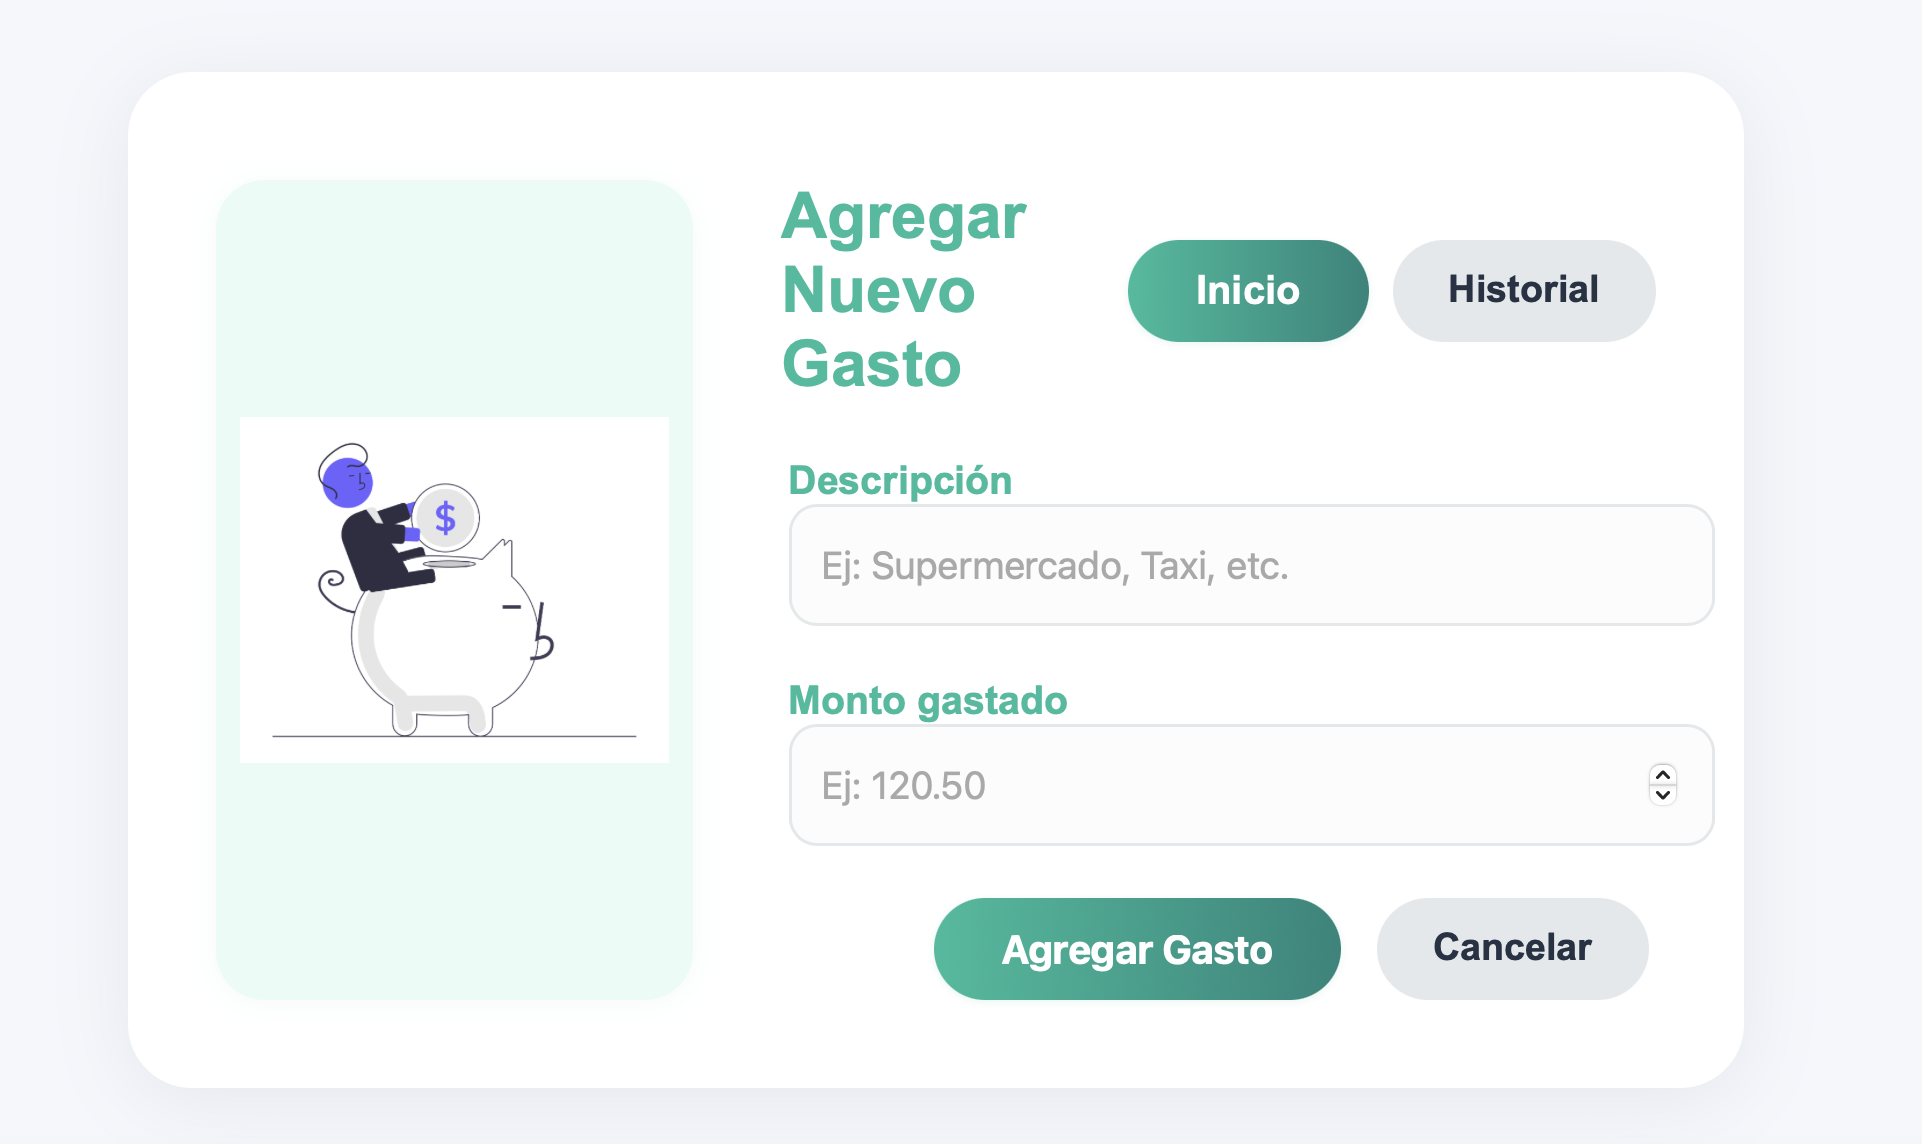
\includegraphics[width=0.8\textwidth]{Imagenes/Formulario.png}
\end{lstlisting}

\section{Evidencia visual de funcionamiento}

\begin{figure}[H]
    \centering
    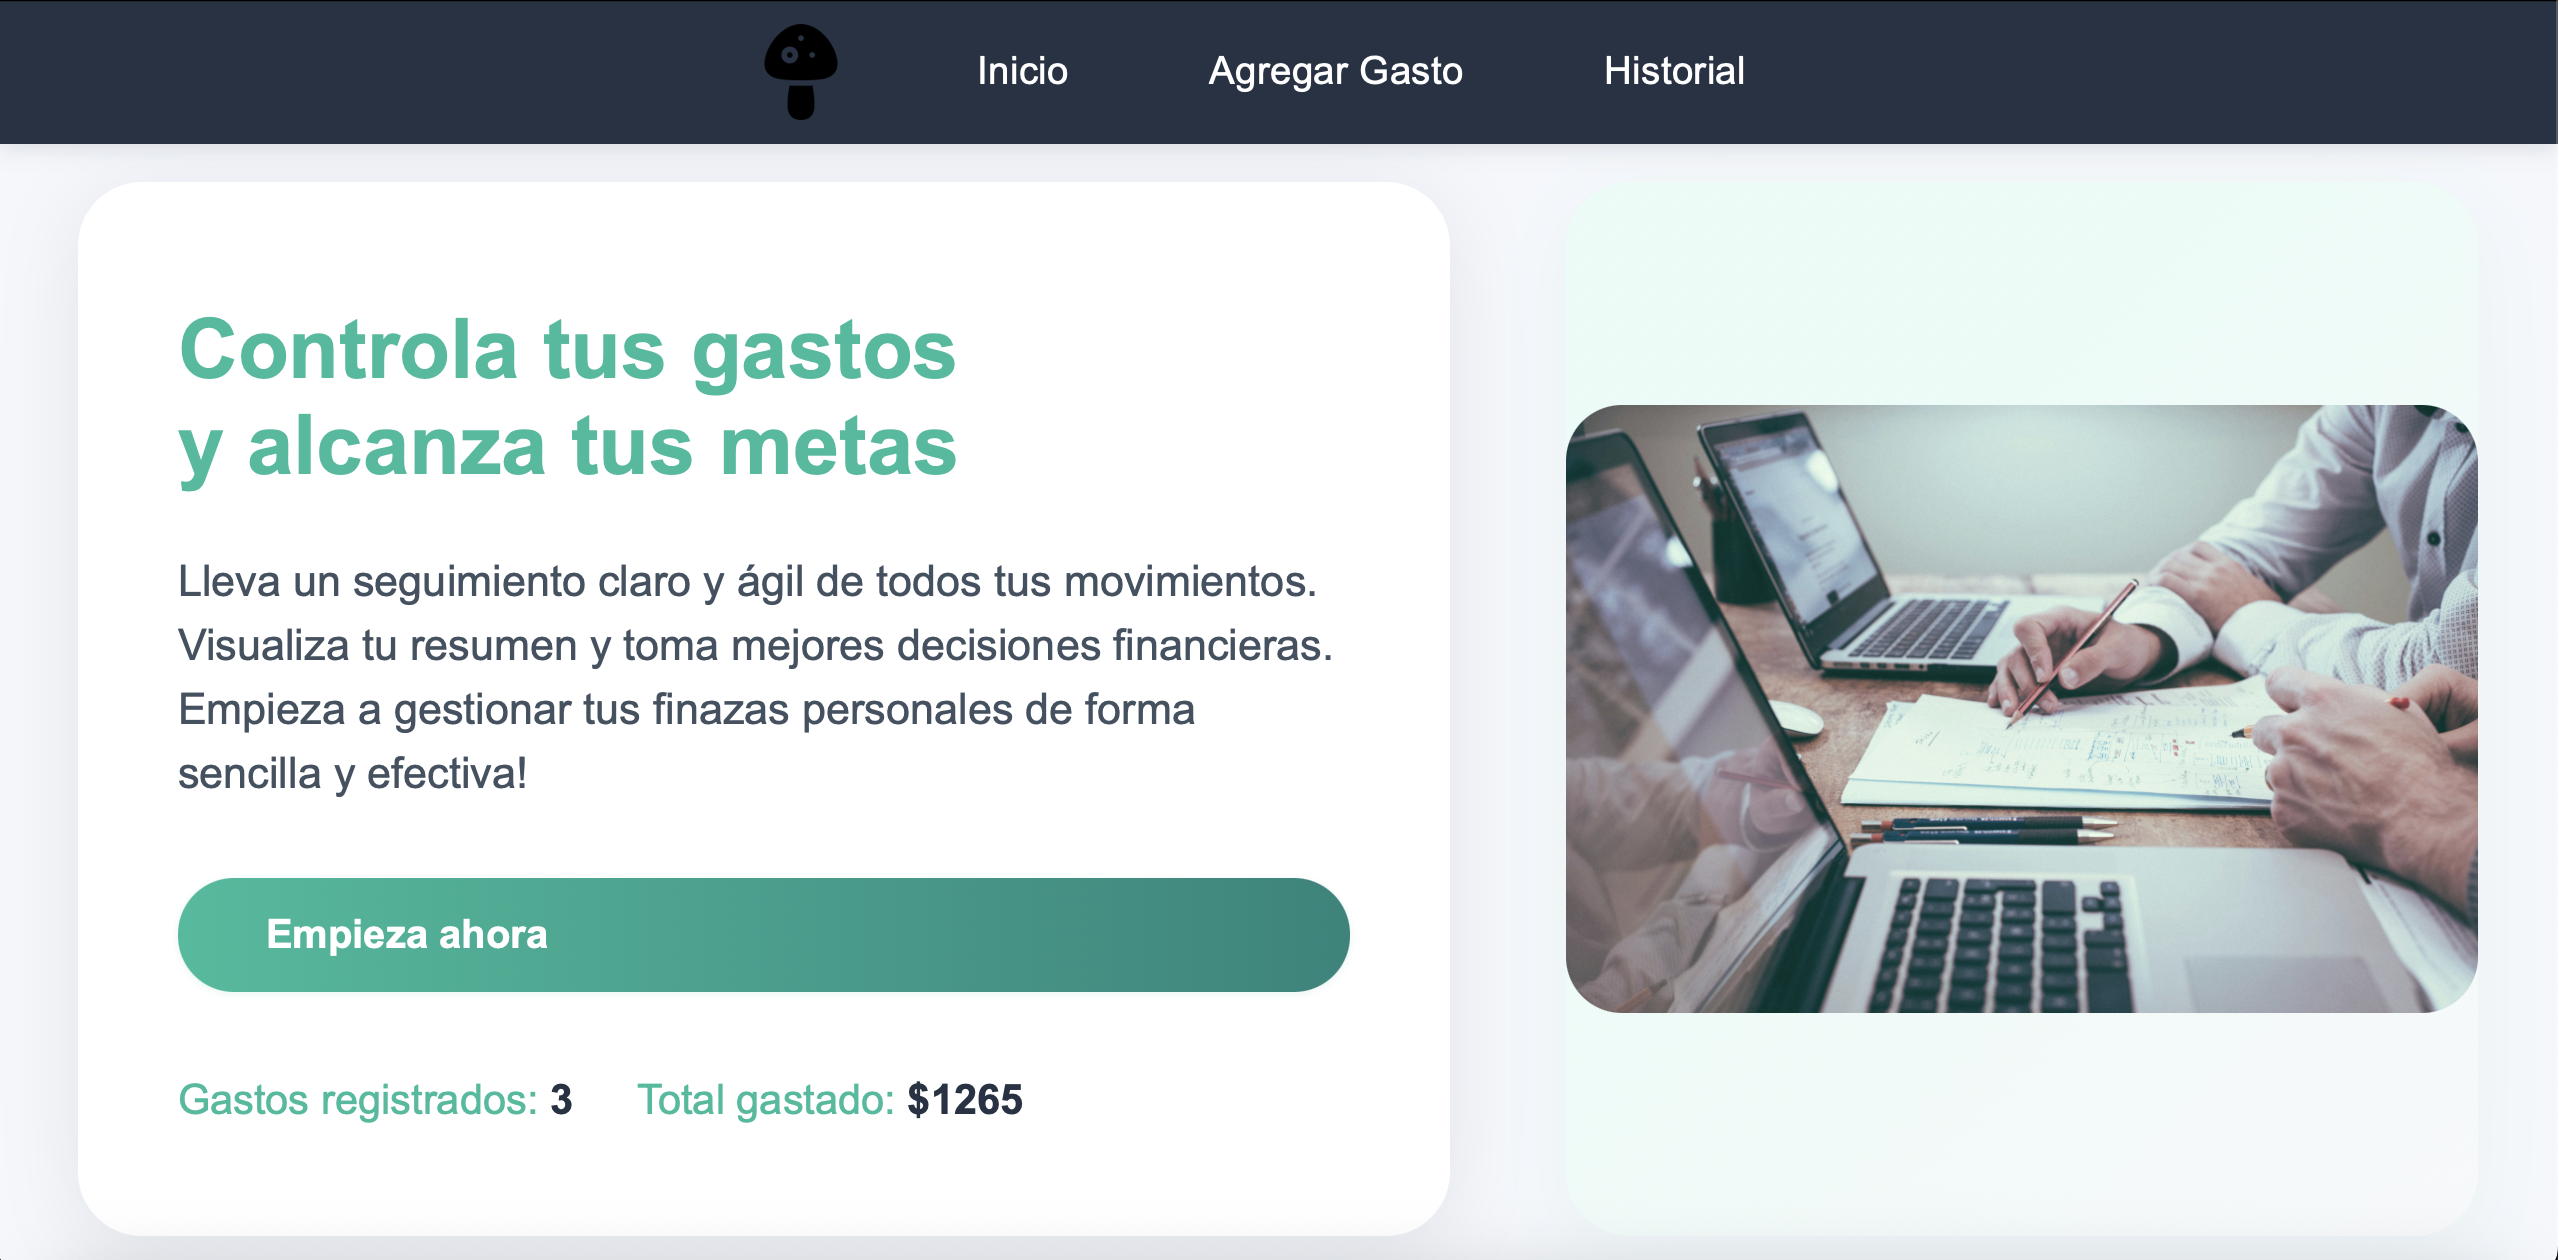
\includegraphics[width=0.85\textwidth]{Imagenes/Pagina Principal.png}
    \caption{Página principal o landing}
\end{figure}

\begin{figure}[H]
    \centering
    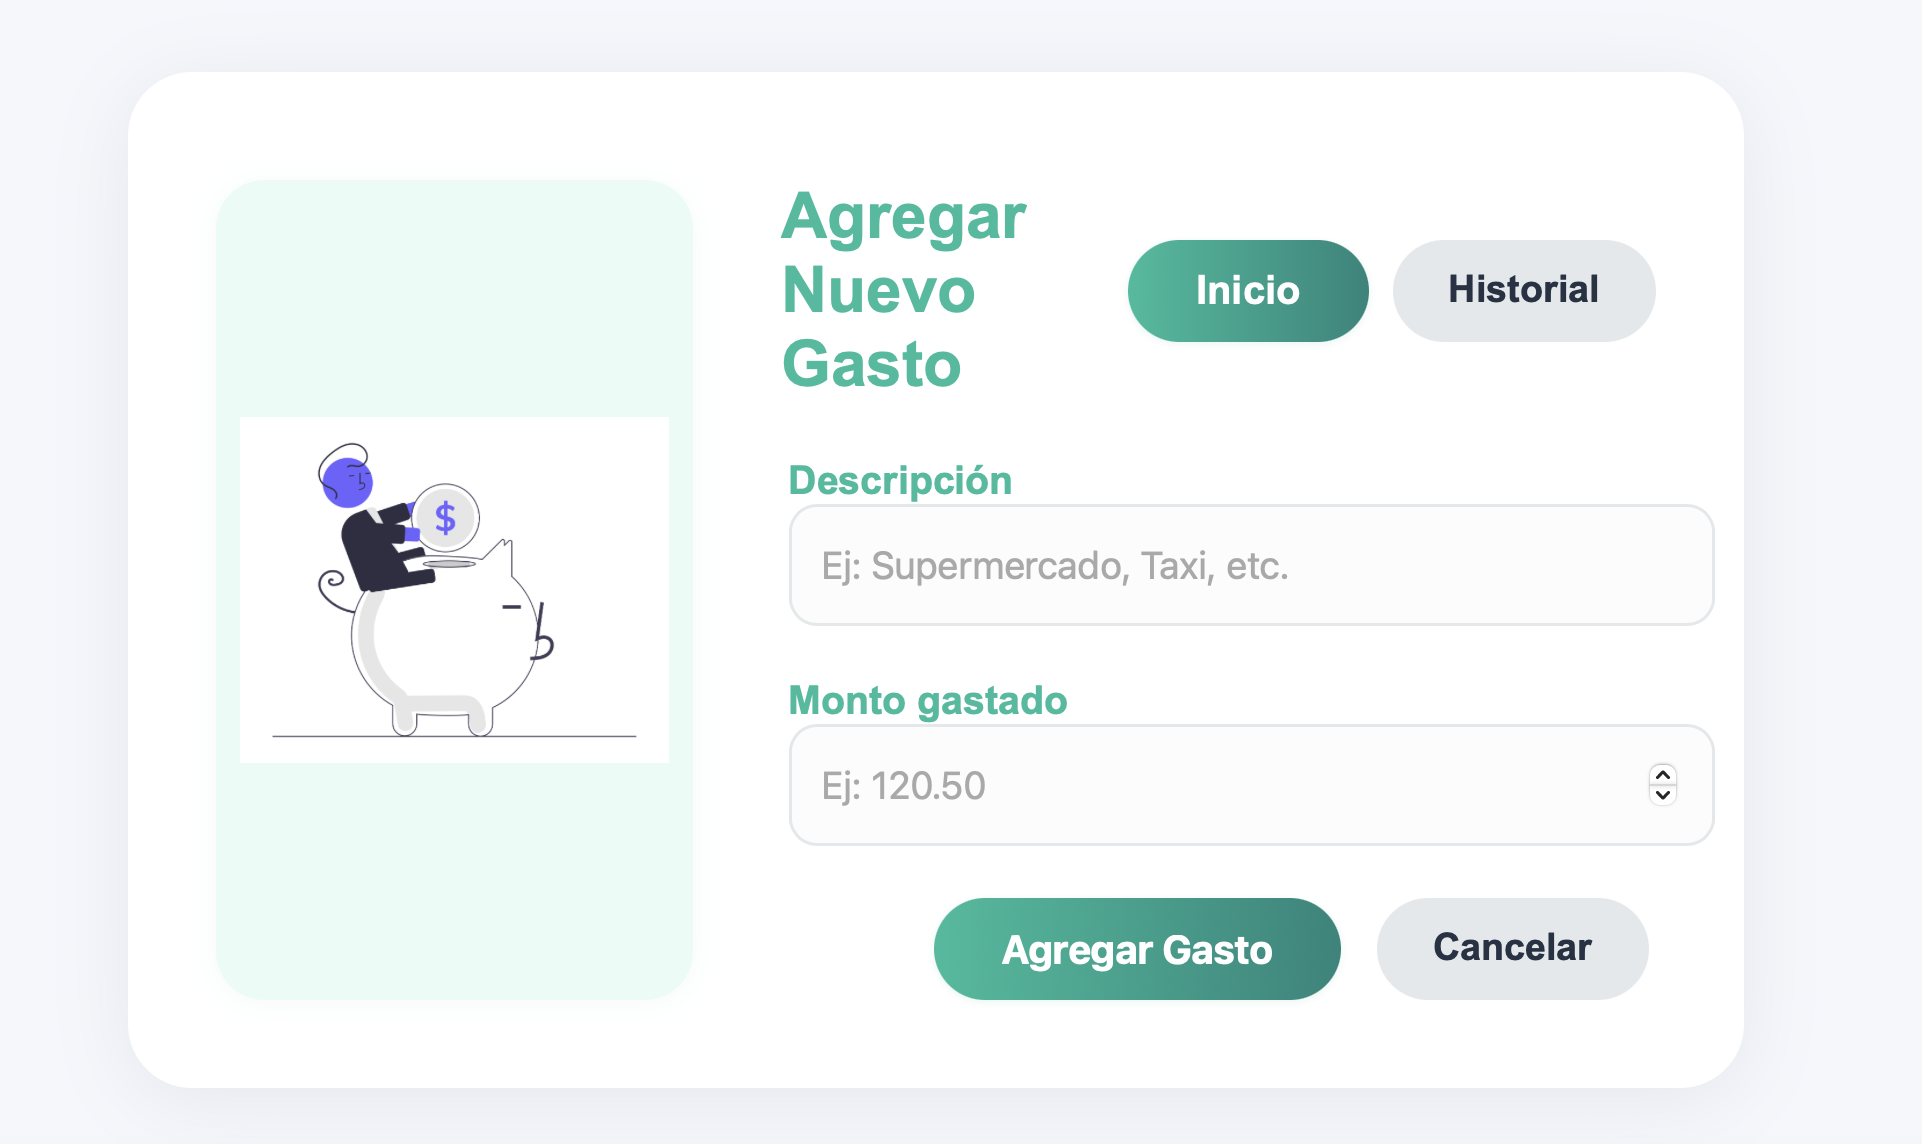
\includegraphics[width=0.85\textwidth]{Imagenes/Formulario.png}
    \caption{Formulario para agregar gastos}
\end{figure}

\begin{figure}[H]
    \centering
    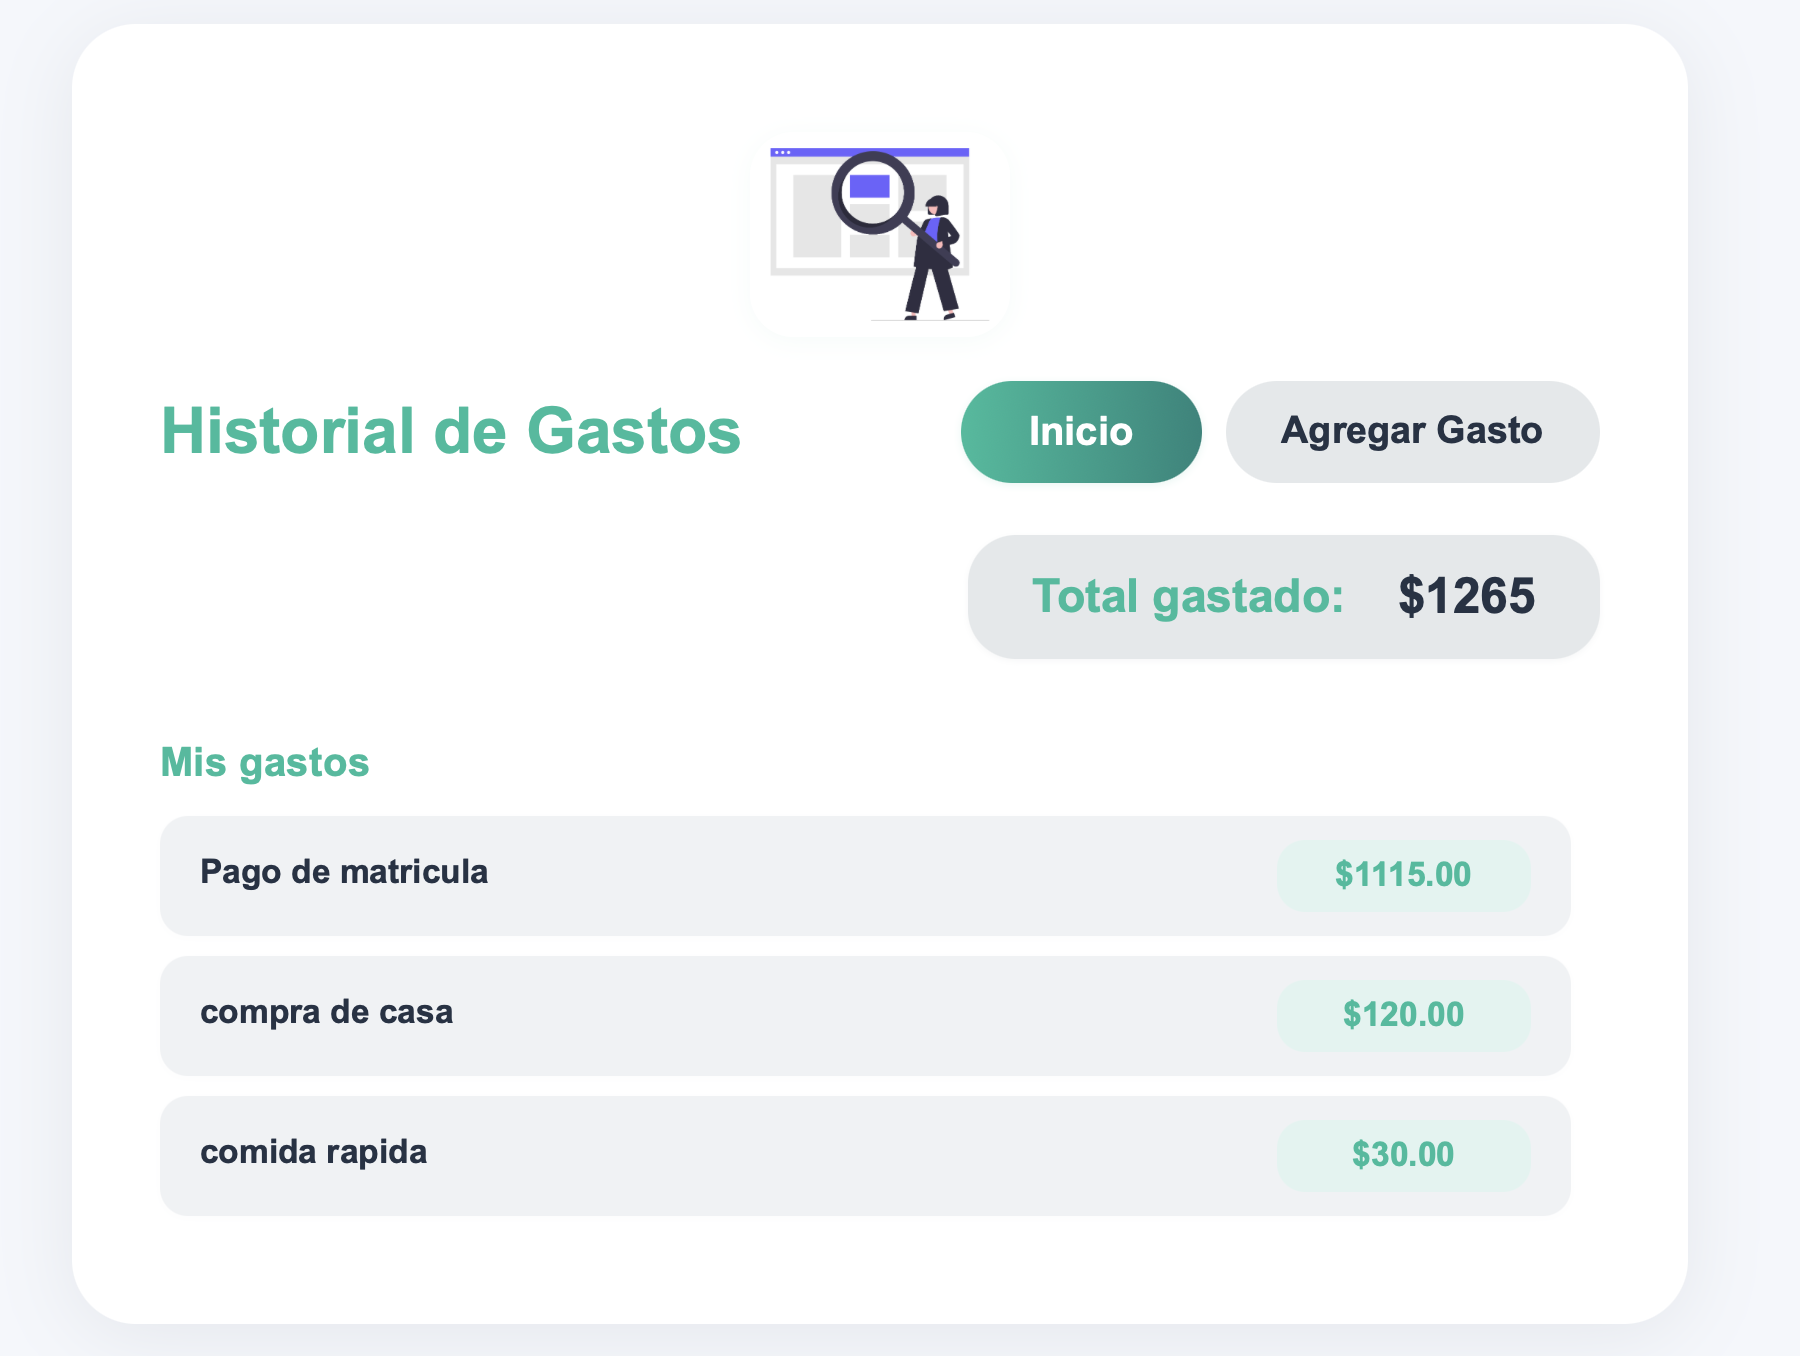
\includegraphics[width=0.75\textwidth]{Imagenes/Historial de gastos.png}
    \caption{Historial de gastos}
\end{figure}

\section{Solución de problemas comunes}
\begin{itemize}
    \item Si ves un error de pip: \texttt{python -m pip install --upgrade pip}
    \item Si el servidor no inicia, verifica estar dentro del entorno virtual (\texttt{.venv} debe estar activado).
    \item Si copiando código se rompe la indentación, corrígela en tu editor.
    \item Si cambiaste modelos, ejecuta siempre:
    \begin{lstlisting}[language=bash]
    python manage.py makemigrations
    python manage.py migrate
    \end{lstlisting}
    \item Si cambias código Python, reinicia el servidor con \texttt{CTRL+C} y luego \texttt{python manage.py runserver}
\end{itemize}

\section{Desactivar el entorno virtual}
Cuando termines, puedes salir del entorno virtual con:
\begin{lstlisting}[language=bash]
deactivate
\end{lstlisting}

\section{¡Consejos para una réplica exitosa!}
\begin{itemize}
    \item Sigue el orden de los pasos, no saltes ninguno.
    \item Usa siempre el entorno virtual.
    \item Verifica la indentación al copiar código.
    \item Si algo falla, lee con calma los mensajes de error, suelen indicar la línea o el archivo con el problema.
    \item Haz pruebas después de cada cambio importante.
\end{itemize}

\section{Conclusión}
Seguir este manual garantiza que cualquier usuario, sin importar su experiencia previa, pueda crear el sistema “Mis Gastos” tal como fue planeado, logrando una aplicación funcional, ordenada y visualmente agradable. Si surgen errores, revisa cuidadosamente cada paso, comando y archivo.

\vfill
\begin{center}
    \textbf{ Fin del Manual }
\end{center}

\end{document}